\section{Partial Dependence Plots}

\begin{frame}[c]
\Huge{\centerline{Partial Dependence Plots}}
\end{frame}
%----------------------------------------------------------------------------------------

\begin{frame}\frametitle{Review of Marginal Expectation}
	\begin{itemize}
		\item Recall that in a $P$-dimensional feature space, we can consider a single feature $X_j \in \mathcal{P}$ and its complement set $\mathcal{P}_{(-j)}$ (where $\{X_j\} \cup \mathcal{P}_{(-j)} = \mathcal{P}$). 
		\item To describe the partial dependence $g(\mathbf{X})$ on $X_j$, we go through the following enumerated explanation:
		\begin{enumerate}
			\item Expected value is $\mathbb{E}[g\mathbf(X)] = \displaystyle\sum_{i = 0}^{N-1}g(x^{(i)})p(x^{(i)})$.
			\item  Let $g(\mathbf{X}) = g(X_j, X_{(-j)})$ and set $X_j = [x_{j}^{0}, \dots, x_{j}^{P-1}]^T)$. 
			\item Then the marginal expectation over $X_{(-j)}$ is $\mathbb{E}_{X_{(-j)}}\left[g(X_j, X_{(-j)})\right] =  \displaystyle\sum_{i = 0}^{N-1} g(X_j, X_{(-j)}) p(x^{(i)})$.
			\item Given that  $\displaystyle\sum_{i = 0}^{N-1} p(x^{(i)}) = 1$, and equal probabilities, $p(x^{(i)}) = \frac{1}{N}$.
			\item Thus $\mathbb{E}_{X_{(-j)}}\left[g(X_j, X_{(-j)})\right] = \displaystyle\frac{1}{N}\sum_{i = 0}^{N-1}g(x_j, \mathbf{x}_{(-j)}^{(i)})$.
		\end{enumerate}
	\end{itemize}
\end{frame}

%----------------------------------------------------------------------------------------

\begin{frame}\frametitle{Partial Dependence Plots (Cont.)}
	\begin{itemize}
	\item The partial dependence of a given feature $X_j$ is the average of the response function $g$, where all the components of $X_j$ are set to $x_j$ $(X_j= [x_j^{(0)}, \dots, x_j^{(N-1)}]^T)$, and all other feature vectors of the complement set $\mathbf{x}_{(-j)}^{(i)}$ are left as the original dataset specified.
	\item Thus, the \textit{one-dimensional partial dependence} of a function $g$ on  $X_j$ is the marginal expectation:
			\begin{equation}\label{eq:pd1}
			\begin{aligned}
				\text{PD}(X_j, g) &= \mathbb{E}_{X_{(-j)}}\left[g(X_j, X_{(-j)})\right]\\
			&= \frac{1}{N}\sum_{i = 0}^{N-1}g(x_j, \mathbf{x}_{(-j)}^{(i)})
		\end{aligned}
		\end{equation}
	\end{itemize}
\end{frame}

%----------------------------------------------------------------------------------------


\begin{frame}\frametitle{Partial Dependence Plots (Cont.)}		
	\begin{itemize}
		\item Partial dependence plots show the partial dependence as a function of \textit{specific values} of our feature subset.
		\item The plots show how machine-learned response functions change based on the values of an input feature of interest, while taking nonlinearity into consideration and averaging out the effects of all other input features.
		\item Partial dependence plots enable increased transparency in $g$ and enable the ability to validate and debug $g$ by comparing a feature's average predictions across its domain to known standards and reasonable expectations. 
	\end{itemize}
\end{frame}

%----------------------------------------------------------------------------------------

\begin{frame}
\frametitle{Conceptual Example}
\begin{figure}
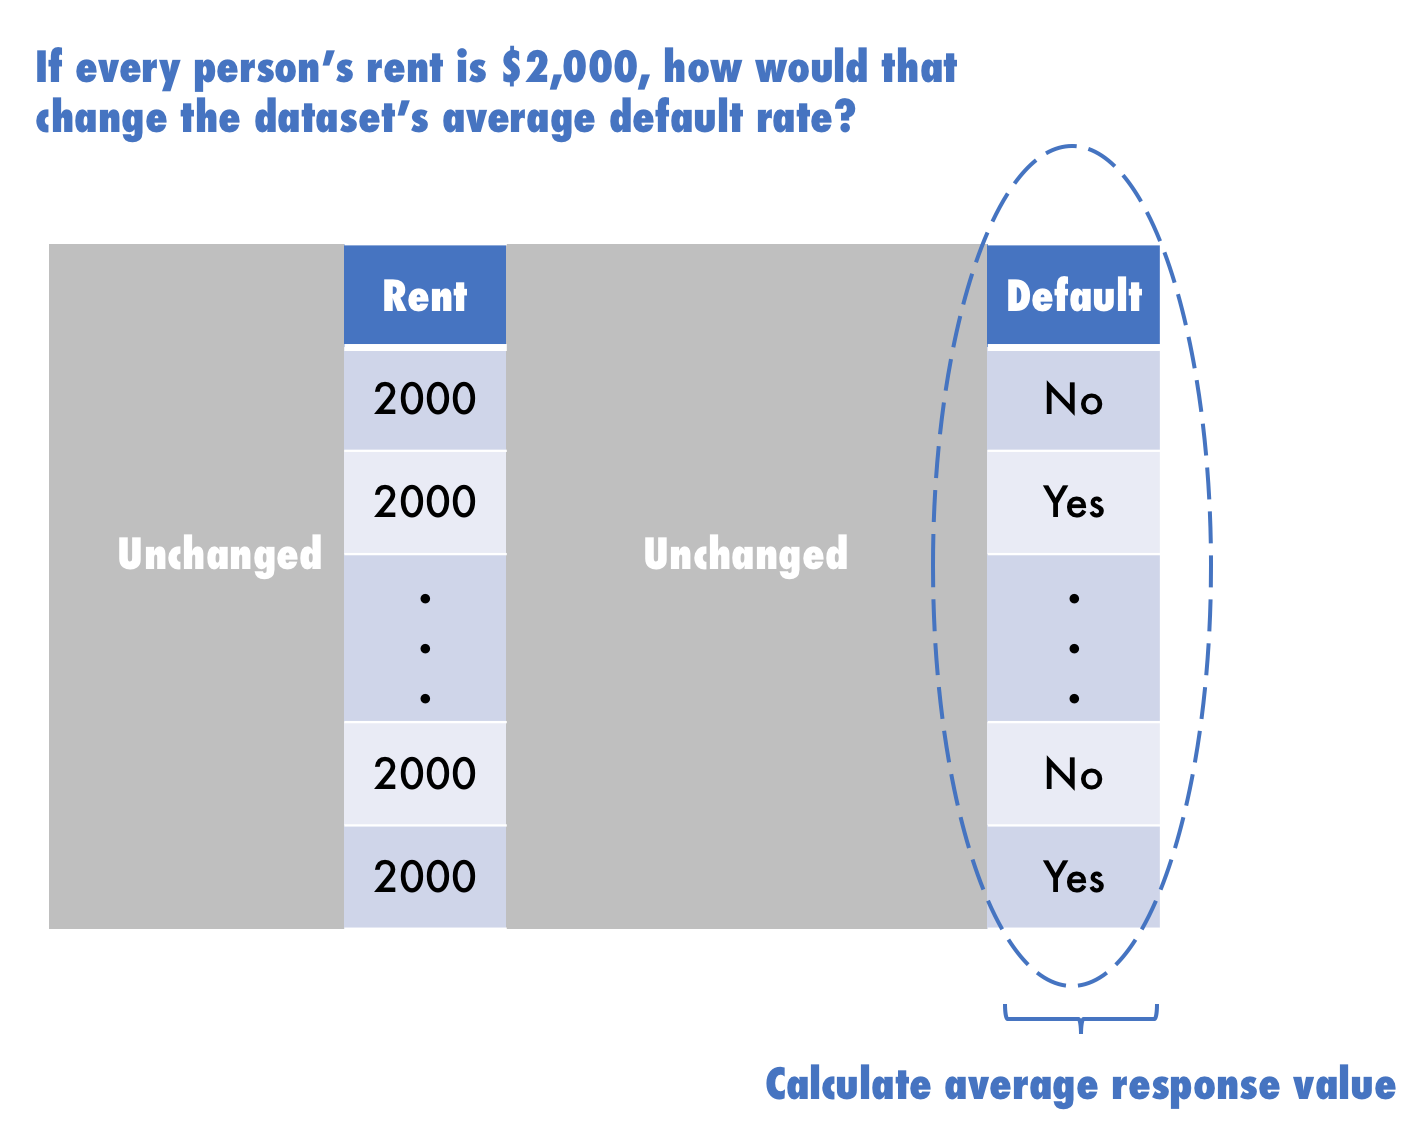
\includegraphics[scale=0.25]{images/pdp_image.png}
\caption{We want to predict whether someone will default on their monthly utility bill. The image shows one feature that we fixed ($Rent=2000$), keeping the rest unchanged, to see its impact on the dataset's average default rate.}
\end{figure}
\end{frame}